\typeout{ ====================================================================}
\typeout{ this is file main.tex, created at 21-Nov-2014               }
\typeout{ maintained by Gustavo Rabello dos Anjos                             }
\typeout{ e-mail: gustavo.rabello@gmail.com                                   }
\typeout{ ====================================================================}

\documentclass[a4paper,portuges,12pt]{article}
\usepackage{babel,varioref,floatflt,wrapfig}
\usepackage{amsmath,booktabs}
\usepackage[utf8]{inputenc}
\usepackage[T1]{fontenc}   % Font Encoding T1 - caracteres acentuados.
\usepackage[top=2cm,bottom=2cm,left=2cm,right=2cm]{geometry}
\usepackage{graphicx}    % pacote para inclusao de figuras,
\usepackage{subfig}
%\pagestyle{empty}
\newcommand{\HRule}{\rule{\linewidth}{0.5mm}}

% removing reference name
\usepackage{etoolbox}
\patchcmd{\thebibliography}{\section*{\refname}}{}{}{}

%%%%%%%%%%%%%%%%%%%%%%%%%%%%%  MACROS MATEMATICOS %%%%%%%%%%%%%%%%%%%%%%%%%%%%%
\newcommand{\tr}{{\,\rm tr}\,}
\newcommand{\sen}{{\,\rm sen}\,}
\newcommand{\senh}{{\,\rm senh}\,}
\newcommand{\diverg}{{\,\rm div}\,}
\newcommand{\grad}{\,\mathbf{grad}\,}
\newcommand{\rot}{\,\mathbf{rot}\,}
\newcommand{\uvet}{\mathbf{u}}
\newcommand{\vvet}{\mathbf{v}}
\newcommand{\wvet}{\mathbf{w}}
\newcommand{\cvet}{\mathbf{c}}
\newcommand{\xvet}{\mathbf{x}}
\newcommand{\gvet}{\mathbf{g}}
\newcommand{\fvet}{\mathbf{f}}
\newcommand{\nvet}{\mathbf{n}}
\newcommand{\tvet}{\mathbf{t}}
\newcommand{\Imat}{\mathbf{I}}
\newcommand{\Eo}{\mathrm{Eo}}
\newcommand{\N}{\mathrm{N}}
\newcommand{\Mo}{\mathrm{Mo}}
%%%%%%%%%%%%%%%%%%%%%%%%%%%%%  MACROS MATEMATICOS %%%%%%%%%%%%%%%%%%%%%%%%%%%%%
										    
\begin{document}	
\typeout{ ====================================================================}
\typeout{ this is file title.tex, created at 21-Nov-2014               }
\typeout{ maintained by Gustavo Rabello dos Anjos                             }
\typeout{ e-mail: gustavo.rabello@gmail.com                                   }
\typeout{ ====================================================================}

\begin{titlepage}
\begin{center}

% Upper part of the page. The '~' is needed because \\
% only works if a paragraph has started.

\includegraphics[width=0.2\textwidth]{./figs/uerj.png}~\\[1cm]

\includegraphics[width=0.3\textwidth]{./figs/gesar.png}~\\[1cm]

\textsc{\LARGE Universidade do Estado do Rio de Janeiro}\\[1.5cm]

\textsc{\Large Relatório Atividades -- CAPES}\\[0.5cm]

% Title
\HRule \\[0.4cm]
{ \huge \bfseries Sistema de Simulação Numérica de Escoamentos
Multifásicos\\[0.4cm] }
{ \Large \bfseries Projeto: A067/2013\\[0.4cm] }
\HRule \\[1.0cm]

% Author and supervisor
\noindent
\large
\emph{Bolsista de Iniciação Científica:}\\
Vinícius A. C. \textsc{Mascarenhas}\\
\vspace{0.3cm}
\emph{Bolsista Jovem Talento:}\\
Gustavo R. \textsc{Anjos}\\
\vspace{0.3cm}
\emph{Coordenador:}\\
Norberto \textsc{Mangiavacchi}\\
\vfill

% Bottom of the page
{\large \today}

\end{center}
\end{titlepage}

\typeout{ ****************** End of file title.tex ****************** }



\section{Identificação}

\noindent Dados do Coordenador: 
\begin{itemize}
	\item \textbf{Nome:} Norberto Mangiavacchi
	\item \textbf{CPF:} 732.841.227-53
	\item \textbf{Escolaridade:} Doutorado
	\item \textbf{Endereço Profissional:} Rua Fonseca Teles, 121 --
	Prédio Anexo, CEP 20940-903 São Cristóvão, RJ - Rio de Janeiro
	\item \textbf{Telefone Profissional:} +55 21 2332-4733
	\item \textbf{Endereço Eletrônico:} {\tt norberto@uerj.br}, 
	                                    {\tt norberto.mangiavacchi@gmail.com}
	\item \textbf{Página Profissional:} {\tt http://www.gesar.uerj.br}
\end{itemize}

\hspace{1cm}

\noindent Dados do Bolsista de Inicação Científica: 
\begin{itemize}
	\item \textbf{Nome:} Vinícius Augusto Cinquini Mascarenhas
	\item \textbf{CPF:} 143.776.267-01
	\item \textbf{Escolaridade:} 2o. grau
	\item \textbf{Endereço Profissional:} Rua Fonseca Teles, 121 --
	Prédio Anexo, CEP 20940-903 São Cristóvão, RJ - Rio de Janeiro
	\item \textbf{Telefone Profissional:} +55 21 2332-4733
	\item \textbf{Endereço Eletrônico:} {\tt vinicius.mascarenhas@icloud.com}
	\item \textbf{Página Profissional:} {\tt http://www.gesar.uerj.br}
\end{itemize}

\clearpage

\section{Resumo}
Após um ano completo do projeto CAPES - Bolsa de Atração de Jovens
Talentos, os objetivos e metas previstos para o primeiros período foram
realizados com sucesso. Este documento apresenta o relatório de
atividades do aluno bolsista de iniciação científica Vinícius Augusto
Cinquini Mascarenhas no projeto entitulado "Sistema de Simulação
Numérica de Escoamentos Multifásicos -- A067/2013", sob supervisão do
Bolsista JVT Gustavo Rabello dos Anjos e Prof. Norberto Mangiavacchi. 
\clearpage

\section{Introdução}
Deseja-se abordar o desenvolvimento e o estudo numérico de dois
problemas atuais como continuidade de projetos de pesquisa e
desenvolvimento realizados na Universidade do Estado do Rio de
Janeiro/GESAR: 

\begin{itemize}
\item Sistema de simulação numérica de produção, estocagem,
transporte e consumo de metano da decomposição de biomassa em
reservatórios de hidrelétricas (Edital FAPERJ 09/2013 – Programa de
apoio às engenharias 2013); 
\item Simulação numérica de estrutura de
não-equilíbrio em sistemas químicos, biológico e ambientais (Edital de
Cooperação Internacional – Chamada Bilateral CNPq 17/2013 – Bélgica).
\end{itemize}

Ambos com suporte técnico-científico do simulador de escoamentos
multifásicos escrito em linguagem orientada a objetos (MATLAB/C++)
utilizando moderna discretização das equações de governo através do
método de elementos finitos. Para execução do projeto proposto,
planeja-se concluir o desenvolvimento do simulador para modelos
tridimensionais e axisimétricos através da incorporação das seguintes
características: paralelização dos núcleos de cálculo intensivo em
clusters baseados em processadores de vários núcleos (multicore),
extensa validação do modelo numérico através de validações analíticas e
experimentais, este último com colaboração internacional, e publicação
dos resultados em canais de comunicação internacionais de excelência.
Com isso, objetiva-se o aperfeiçoamento das técnicas computacionais
empregadas na instituição de execução do projeto (UERJ/GESAR),
consolidando o Programa de Pós-graduação em Engenharia Mecânica na UERJ,
e a formação de recusos humanos, com aperfeiçoamento pessoal de nível
superior e pós-graduação. A participação do aluno bolsista de iniciação
científica é contextualizada em sua inicialização aos procedimentos
laboratoriais, bem como a introdução à realização de procedimentos
acadêmicos, tais como elaboração derelatórios científicos, pesquisa
bibliográfica e artigos acadêmicos.

\section{Objetivos}
\begin{itemize}
	\item estudo e desenvolvimento de modelo simplificado para dinâmica
	      de fluidos computacional;
    \item pesquisa bibliográfica pertinente ao projeto de pesquisa;
	\item familiarização de documentos científicos tais como, relatórios
	      de atividades, procedimentos laboratorias e artigos científicos.
	\item suporte na realização de experimentos computacionais e
		  laboratoriais de decomposição de biomassa e produção de gases
		  com sedimentação de material orgânico; de medição da
		  sedimentação/ressuspensão e consumo de produtos.
\end{itemize}

\section{Atividades Desenvolvidas pelo Bolsista IC}

\begin{itemize}
\item Revisão bibliográfica pertinente ao projeto;
\item familiarização com as técnicas desenvolvidas e implementadas no
código numérico;
\item execução de testes no código numérico;
\item aumento da qualificação profissional do aluno de IC através de
desenvolvimento e pesquisa.
\end{itemize}


\section{Plano de Trabalho}
O plano de trabalho proposto para o período de 4 bimestres de
projeto pode ser encontrado na Fig.(\ref{fig:plano}. Nota-se que o plano de trabalho foi reduzido em
2 bimestres, pois o aluno bolsista de iniciação científica desistiu da
bolsa de estudos e foi substituido pelo aluno Paulo Roberto Berti Leite
Filho, estudante do quinto período de engenharia da Universidade do
Estado do Rio de Janeiro -- UERJ.

 \begin{figure}[ht!]
 	\begin{center}
 		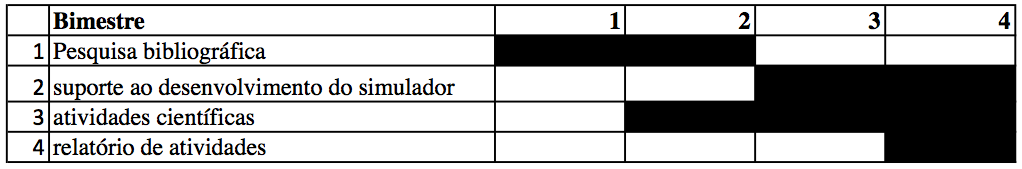
\includegraphics[angle=0, scale=0.9]{figs/ic-plano.png}
 	\end{center}
 	\caption{Plano de trabalho proposto para o período inicial de
	execução do projeto Bolsa de Atração de Jovens Talentos - CAPES para
	o aluno de IC Vinícius Augusto Cinquini Mascarenhas.}
 	\label{fig:plano} 
 \end{figure}

\section{Resultados Obtidos}

A pesquisa bibliográfica foi realizada com sucesso, onde o bolsista
identificou os pontos mais importantes da modelagem matemática e
implementação numérica para suporte na realização do projeto. Alguns
testes pertinentes com o código numérico foram realizados com sucesso em
problemas bidimensionais simples de dinâmica de fluidos computacional.
Alguns testes e validações foram realizados com sucesso ao lado do
pesquisador bolsista Gustavo Rabello dos Anjos e os resultados podem ser
encontrados na seção de Resultados Obtidos no relatório parcial de
atividades do bolsista JVT. É importante notar que o aluno de IC foi
estimulado ao desenvolvimento de pesquisa acadêmcia com intensa
participação em atividades laboratorias realizadas no GESAR/UERJ, bem
como socialização com os demais membros do laboratório, dentre eles
outros alunos de IC, alunos de mestrado, doutorado e professores.

\end{document}	

\typeout{ ****************** End of file main.tex ****************** }

